%%%%%%%%%%%%%%%%%%%%%%%%%%%%%%%%%%%%%%%%%
% FRI Data Science_report LaTeX Template
% Version 1.0 (28/1/2020)
%
% Jure Demšar (jure.demsar@fri.uni-lj.si)
%
% Based on MicromouseSymp article template by:
% Mathias Legrand (legrand.mathias@gmail.com)
% With extensive modifications by:
% Antonio Valente (antonio.luis.valente@gmail.com)
%
% License:
% CC BY-NC-SA 3.0 (http://creativecommons.org/licenses/by-nc-sa/3.0/)
%
%%%%%%%%%%%%%%%%%%%%%%%%%%%%%%%%%%%%%%%%%


%----------------------------------------------------------------------------------------
%	PACKAGES AND OTHER DOCUMENT CONFIGURATIONS
%----------------------------------------------------------------------------------------
\documentclass[fleqn,moreauthors,10pt]{ds_report}
\usepackage[english]{babel}
\usepackage{float} 
\usepackage[section]{placeins}
\graphicspath{{fig/}}




%----------------------------------------------------------------------------------------
%	ARTICLE INFORMATION
%----------------------------------------------------------------------------------------

% Header
\JournalInfo{UL FRI Data Science - Introduction to Data Science, 2021-2022}

% Interim or final report
%\Archive{Interim report}
\Archive{Project 2 Report}

% Article title
\PaperTitle{When companies pay and when cancel?}

% Authors and their info
\Authors{Vito Založnik\textsuperscript{1}}
\affiliation{\textsuperscript{1}\textit{vz9592@student.uni-lj.si, 63210496}}

% Multiple authors
%\Authors{John Doe\textsuperscript{1}, Jane Doe\textsuperscript{2}, and Mike Smith\textsuperscript{3}}
%\affiliation{\textsuperscript{1}\textit{john.doe@fri.uni-lj.si, 63181234}}
%\affiliation{\textsuperscript{1}\textit{jane.doe@fri.uni-lj.si, 63185678}}
%\affiliation{\textsuperscript{1}\textit{mike.smith@fri.uni-lj.si, 63171234}}

% Keywords
\Keywords{Paying, Pql, Filter features}
\newcommand{\keywordname}{Keywords}


%----------------------------------------------------------------------------------------
%	ABSTRACT
%----------------------------------------------------------------------------------------

\Abstract{
In this project report I wanted to get and represent an overview of data and find connection between parameters that could be used in future modeling. Underlying theme of the report is to find if there are any differences between companies that are paying for Databox's services and those who don't. Observations that I have found to be the most interesting are also visualized.
}

%----------------------------------------------------------------------------------------

\begin{document}

% Makes all text pages the same height
\flushbottom

% Print the title and abstract box
\maketitle

% Removes page numbering from the first page
\thispagestyle{empty}

%----------------------------------------------------------------------------------------
%	ARTICLE CONTENTS
%----------------------------------------------------------------------------------------

\section*{Introduction}

    Data exploration is an approach to understand what is in a dataset and the characteristics of the data. These characteristics can include size, completeness of the data, correctness of the data, possible relationships amongst data elements or files/tables in the data. Data exploration is typically conducted using a combination of automated and manual activities.

	Databox company provided us an anonymized and sampled dataset on their platform usage data from last 2 years. Our task was to get brief overview of the data, explore it and visualize some interesting observations. Data was combined from file with signups attributes and files with events. In event files there were quite a lot of data parameters, so it was hard to explore them all.  I decided to focus on exploring if there are some differences between companies that decided to became payable, became pql and those who did not and those who later cancelled subscription. In this report I included only the most interesting observations. Motivation for project was to help company Databox to improve their platform.
	
	


%------------------------------------------------

\section*{Data exploration}
\subsection{Methods}
First I had to do some data preprocessing. I removed some broken rows, added headers to event files and had to change some column types. I also had to divide some parameters from seingle string into list.

From mathematical point of view, the methods that were most used are calculating mean and variance. I also normed some data and calculated a lot of correlations to see possible connections between parameters. For estimating values between discrete data I used polynomial regression as it is unbiased estimator with lowest variance. In last figure I normalized data in respect to relative existing time of each user. This gave better results but the most recent dates seems to be still to sensitive and should be dropped. 
\subsection{Analysis}
First I wanted to get brief overview of how events happened trought time. 

\begin{figure}[H]\centering
	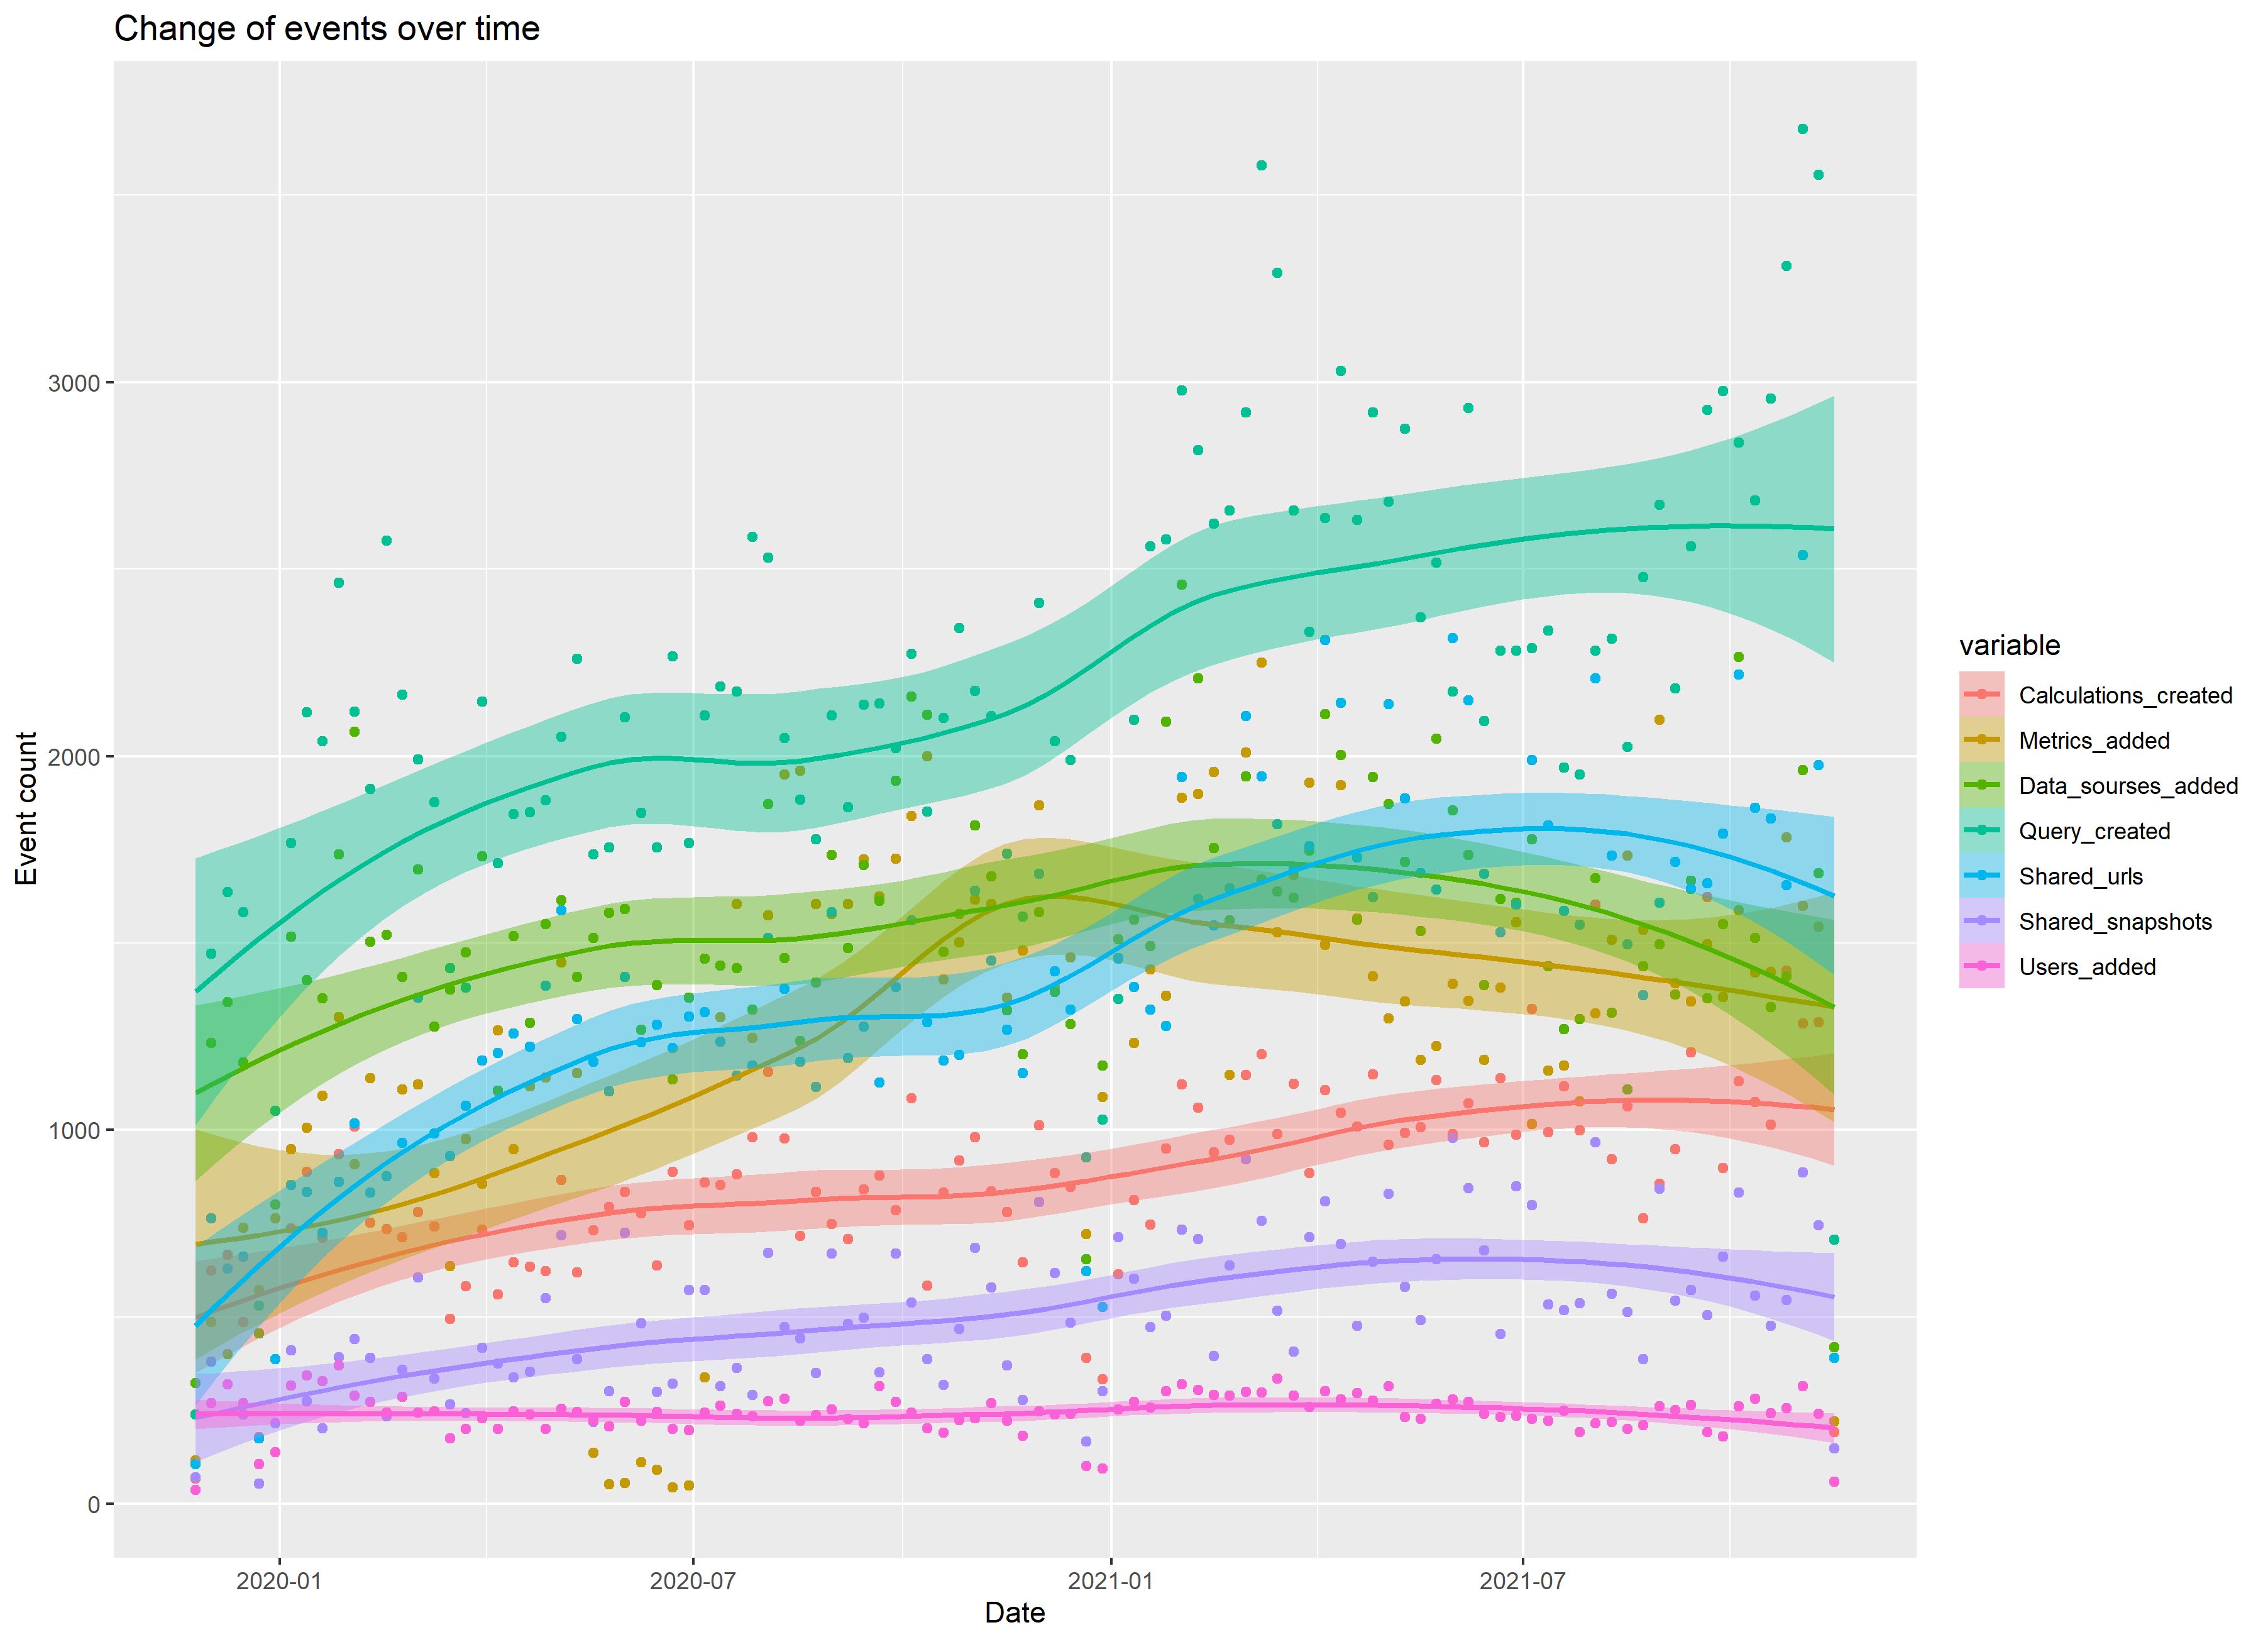
\includegraphics[width=\linewidth]{events_over_time.png}
	\caption{\textbf{Change of events at Databox over time.}  }
	\label{fig:events}
\end{figure}
%Then I calcullated some correlations between signup attributes and compared some groups to each other in hope to find some interesting patterns. 

In Figure 1 we can see how many of each events happened in a single week in the last 2 years and line that is best fit to each event. Number of new added users is the most consistent, as is almost identical at around 300 per week trough all observed period and with least variance. All the other events were in growth but there are some clear drops at certain dates. Biggest drops are at around each New year, when all activities drops significantly. We can also see interesting drop of $metrics\_added$ in the middle of June 2020, which lasted almost a month.

\begin{figure}[H]\centering
	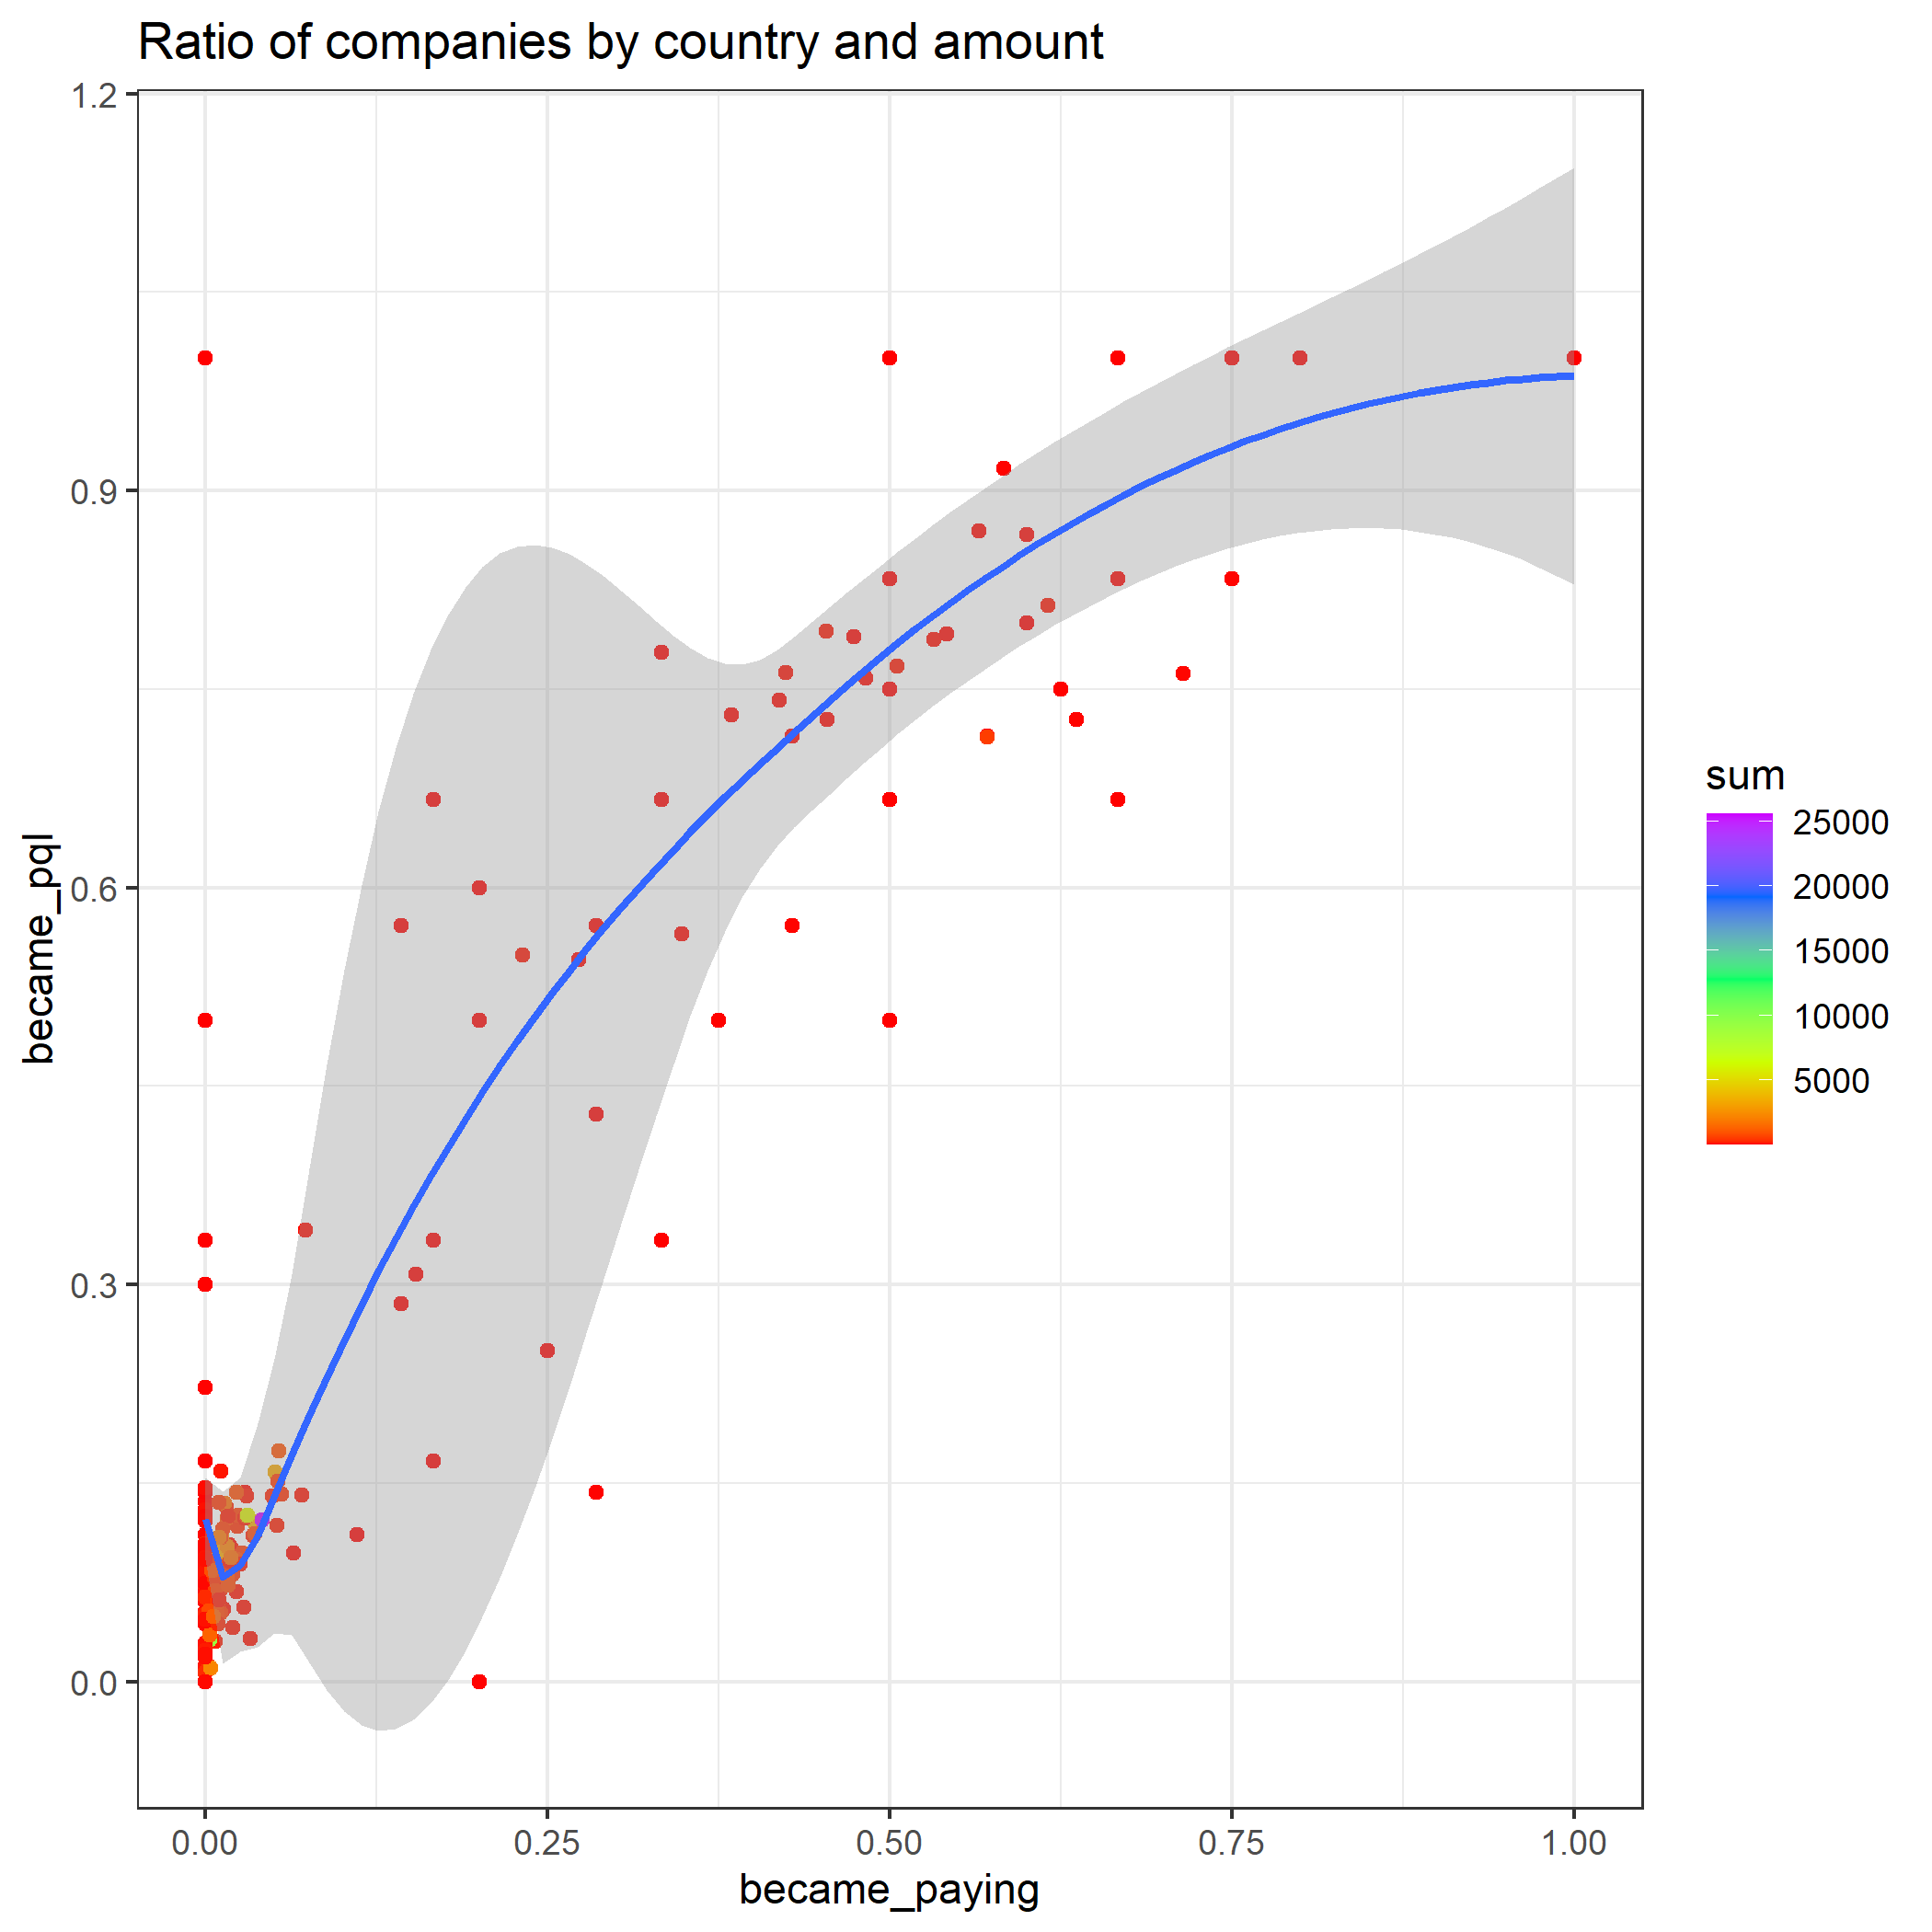
\includegraphics[width=\linewidth]{ratio_paye_pql_county.png}
	\caption{\textbf{Ratio of pql and paying companies in every country}  }
	\label{fig:ratio_pql_paying}
\end{figure}

I was wondering if there are any legal, or other country specific, reasons for companies to start paying or became pql. Colour of every dot represents number of users in every country.  On $y$ axis is ratio of how much of them baceme pql and on $x$ axis is ratio of how much of them became paying. Colour represents the number of users in each country. If an individual country has very small number of users, then ratio is a very unstable indicator. But we can still see a lot of correlation between pql and paying status. We can see some yellow and orange dots not so close to 0, which could be countries with better properties for Databox.
%\subsection*{Tables}

%Use the table environment to insert tables.

%begin{table}[hbt]
%	\caption{Table of grades.}
%	\centering
%	\begin{tabular}{l l | r}
%		\toprule
%		\multicolumn{2}{c}{Name} \\
%		First name & Last Name & Grade \\
%		\midrule
%		John & Doe & $7.5$ \\
%		Jane & Doe & $10$ \\
%		Mike & Smith & $8$ \\
%		\bottomrule
%	\end{tabular}
%	\label{tab:label}
%\end{table}

\begin{figure}\centering
	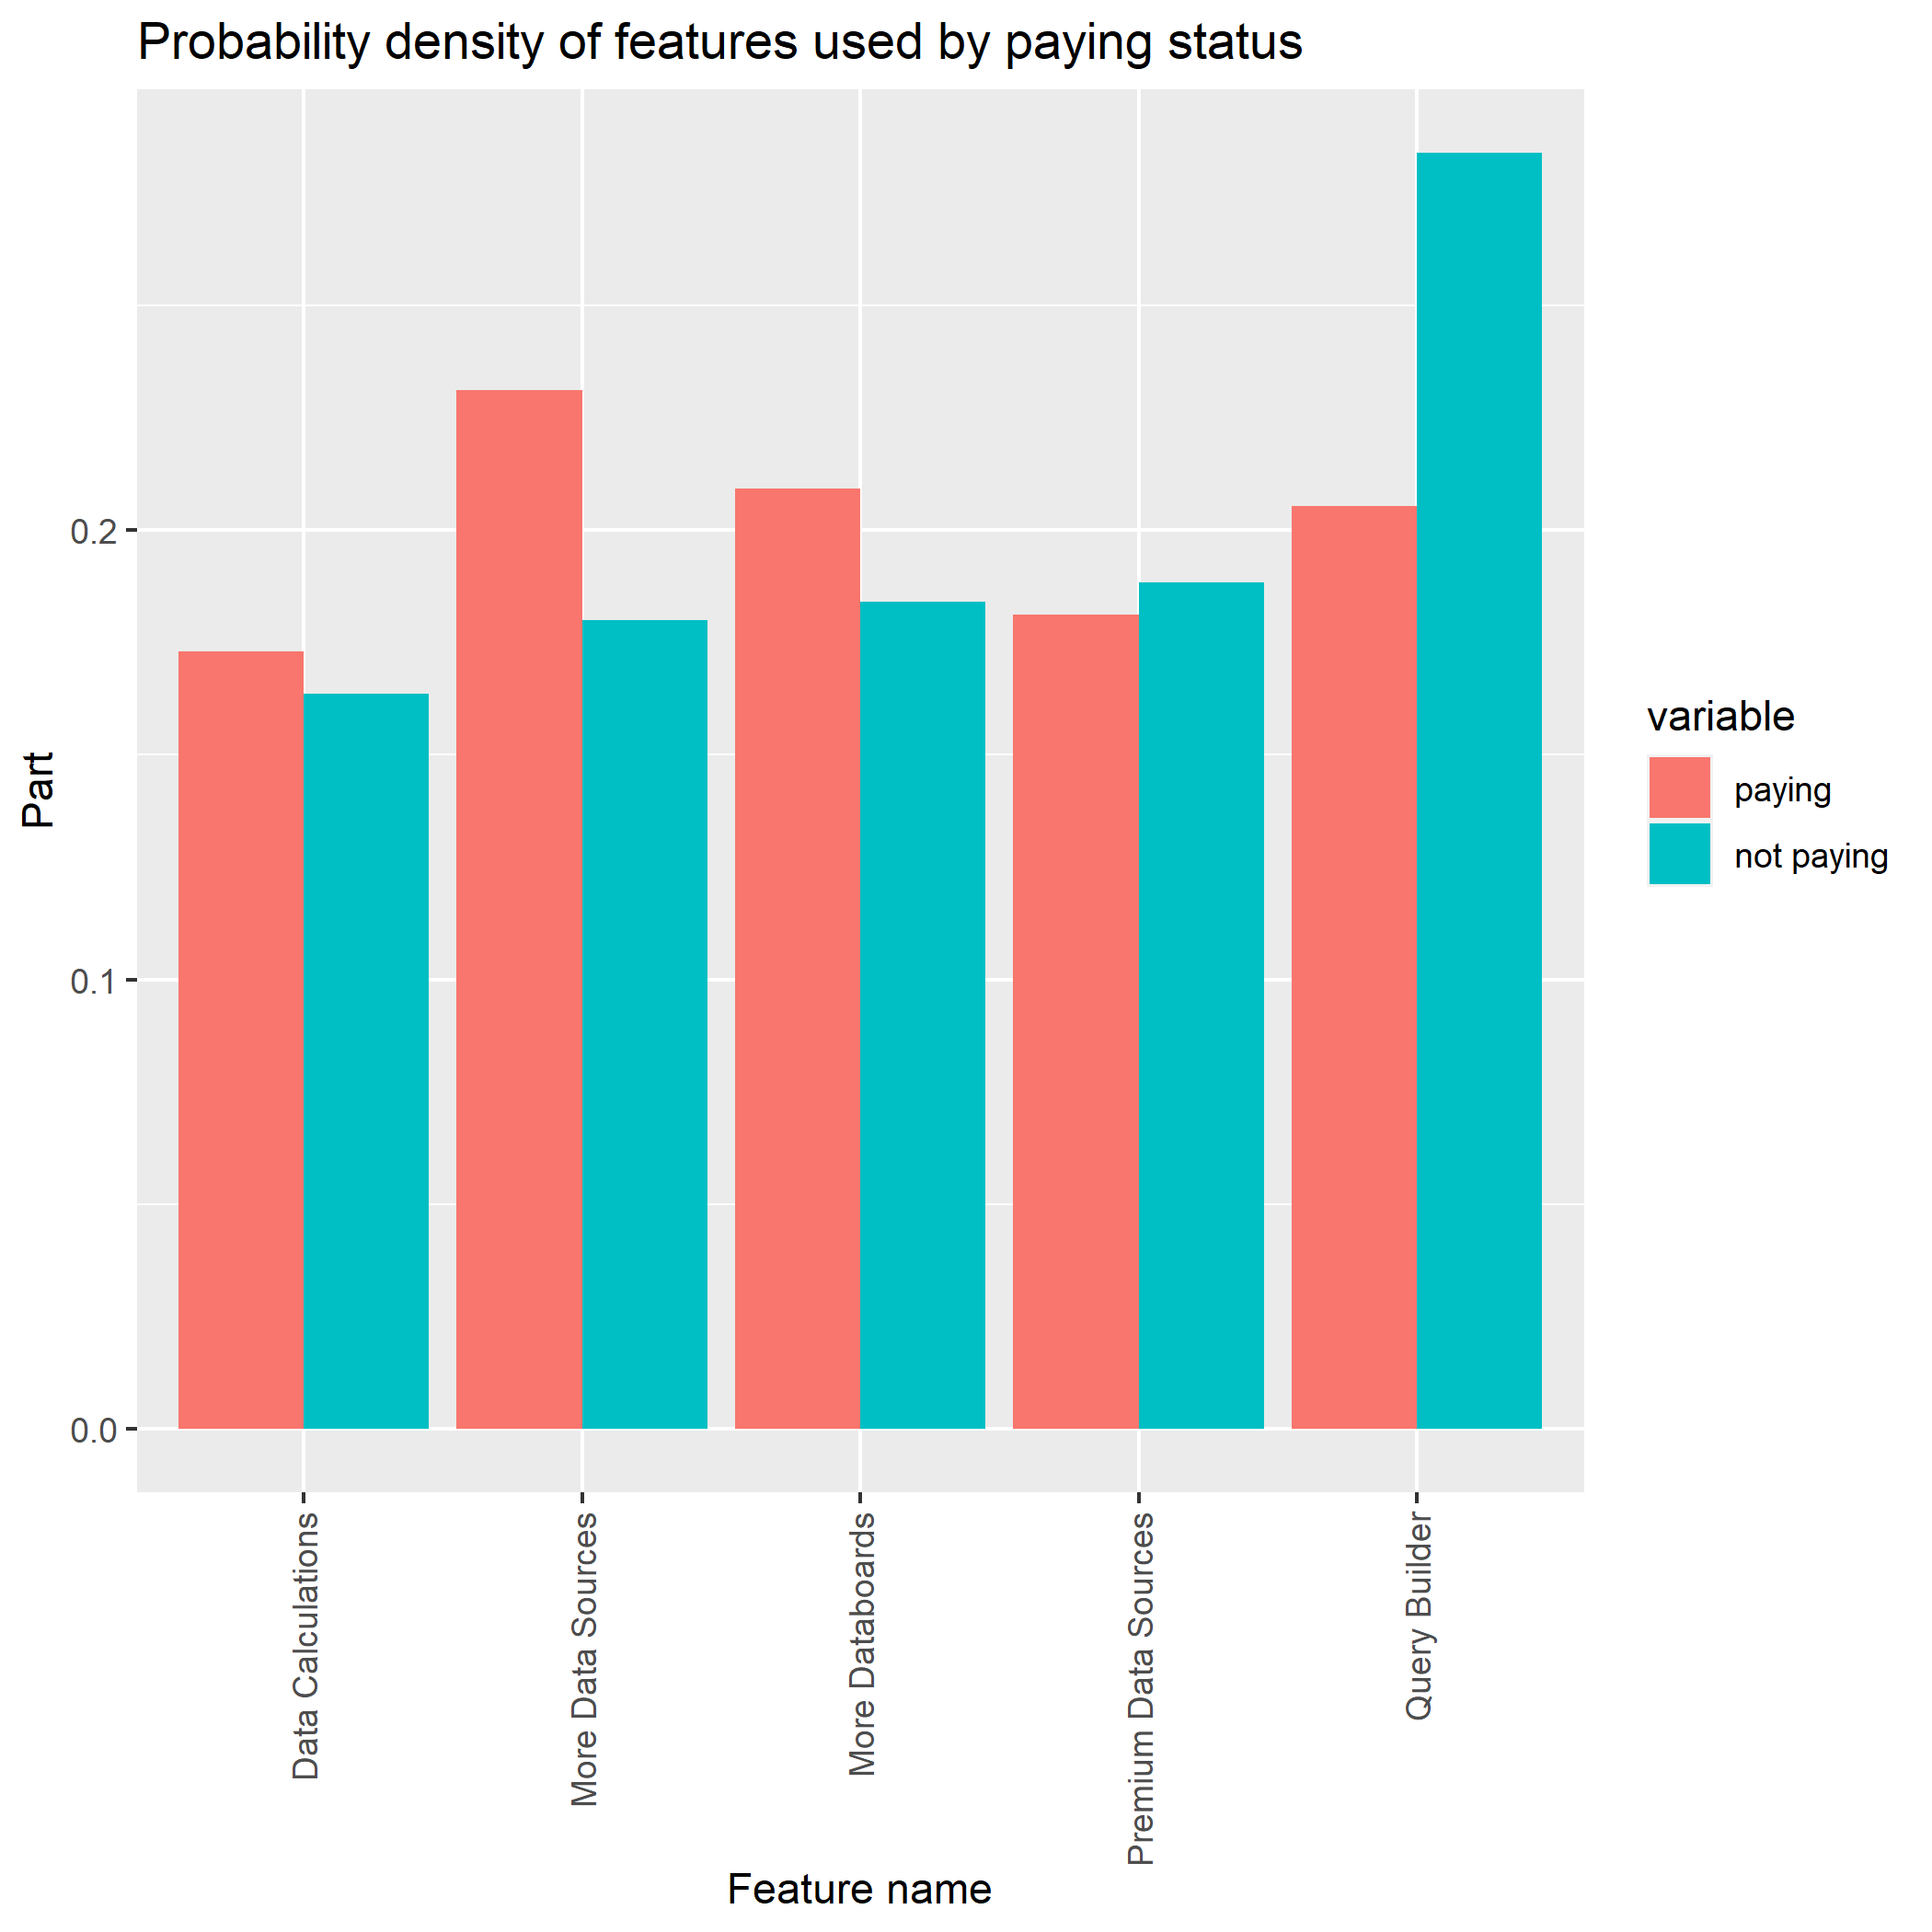
\includegraphics[width=\linewidth]{density_features.png}
	\caption{\textbf{Number of features used in relation to paying status}   }
	\label{fig:trial_features}
\end{figure}
Among those that used trial features we can see there are big differences in usage of each filter in relation to paying status. In group that is not paying there are a lot more users using Query Builder and less other features. In paying group there is a more use of More Data Sources than in non paying.

\begin{figure}\centering
	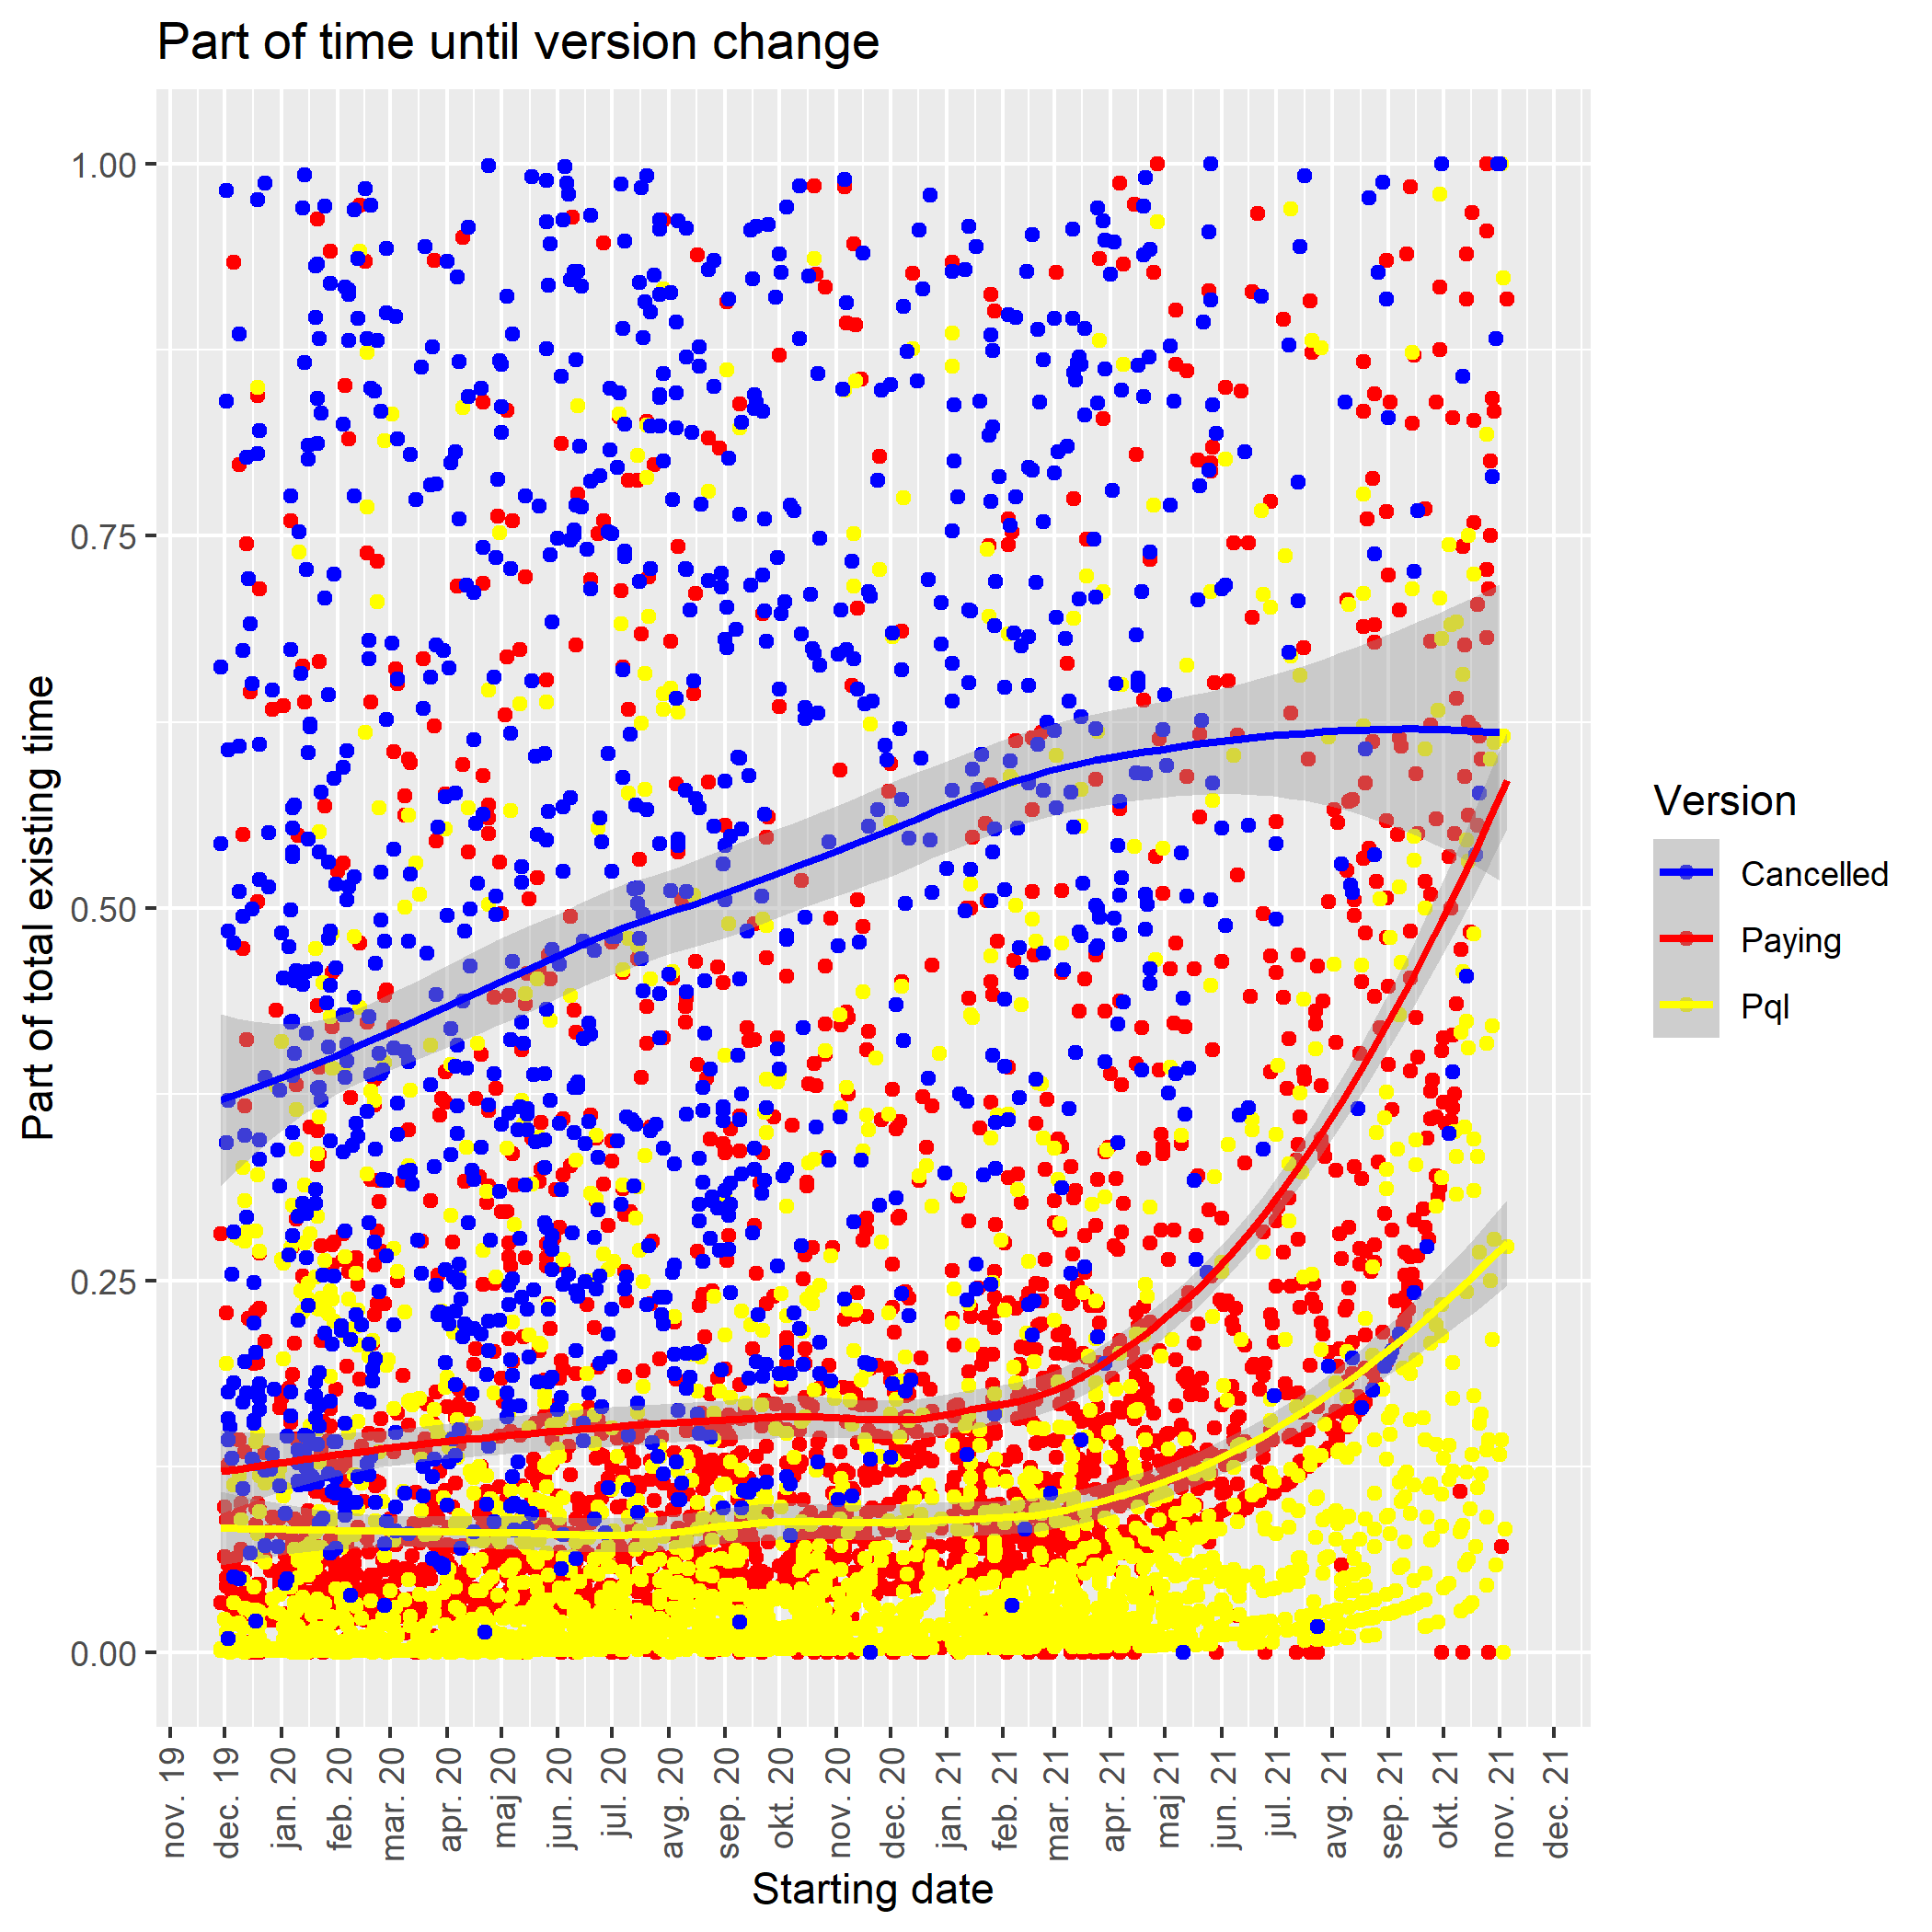
\includegraphics[width=\linewidth]{activity_after_days.png}
	\caption{\textbf{Part of existing time until paying, pql and cancelled among those who started paying} }
	\label{fig:main}
\end{figure}
The main goal of analysis was to find some connection between paying, pql and cancelled status. In figure 4 we can see after what part of existing time each costumer changed his status. On x axis is system creation time of each company that started to pay and on y axis is part of existence until the change of status. Norming of dates was done using formula $\frac{days\_since\_event}{total\_existing\_days}$. Color is specified by version of status change. In the end of time series, data became more and more sensible, so we can see upshift in aproximation curves. But at beginning, especially paying and pql aproximations are quite linear and evenly with constant proportion to each other. This might be used to predict when will company start paying if we know its pql status and when was achieved. 
\begin{center}

\begin{table}
\caption{Figure 4 statistical informations}

\begin{tabular}{|c |c c c||} 
 \hline
  & mean & median & standard deviation \\ [0.5ex] 
 \hline\hline
 pql & 6 & 87837 & 787 \\ 
 \hline
 paying & 7 & 78 & 5415 \\
 \hline
 canceled & 545 & 778 & 7507 \\
 \hline
 
\end{tabular}

%\caption*{The caption without a number}
\end{table}

\end{center}












%------------------------------------------------

\section*{Discussion}

We saw how events changed through time and that there are quite few of drops in all event counts around New year and also some additional drops in just single events. We figured out that pql and paying are very correlated parameters and that there are some differences in trial features used among those who later started paying and those who don't. Interestingly there are also few dompanies that are paying but did not activate subscription. Main observation is, that there is a pattern in elapsed time between change in status from pql to paying. If I would start over again, I would do some grouping by continent rather than only by countries.  I would also try to do some principal component analysis. When norming data for Figure \ref{fig:main} I would rather use only first half of time stamp for reference. But this ideas came too late. This could also be done before project 3 modeling. 





%------------------------------------------------



%----------------------------------------------------------------------------------------
%	REFERENCE LIST
%----------------------------------------------------------------------------------------
%\bibliographystyle{unsrt}
%\bibliography{report}


\end{document}
